\chapter*{Introduction}%\label{Chap:Intro}
This thesis studies the technological and economic implications and requirements of optical network sharing. We propose a solution to enable fine-grained and dynamic inter-operator sharing of the resources using virtualization technology. We show that a carefully designed resource sharing market mechanism can provide sharing incentives for competing operators and enhance the network utilization and value generation. Furthermore, we show how a blockchain-based distributed marketplace for network resources could alleviate the trust issues in conventionally centralized markets. 



% triggered lots of controversy etc and signalled a shift in the main focus of the telcom operators that saw trends such as Netflix a threat to their revenue.


% According to Seward (2014), a journalist, who hints at being an inside
% source, and collaborated by other sources such as Morran (2014), Comcast
% started to “slow” down Netflix’s traffic in 2013 into the Comcast network,
% therefore lowering the quality of Netflix’s streams for Comcast customers. In
% March 2014 a deal signed by Netflix to pay Comcast for not slowing down
% traffic (Morran, 2014; Seward, 2014).
% Netflix is supposed to have similar arrangements in place with Time
% Warner Company, AT\&T and Verizon, i.e. Netflix paying the network operator to not intentionally slow down their traffic, which is supported by Seward
% (2014) and Erickson (2014), both journalists.
% The conflict between Netflix and Comcast is said to have been one of
% the main reasons behind the FCC 2015 ruling enforcing net neutrality in the
% United States, which meant reclassifying ISPs as common carriers under Title
% II (see Wikipedia Contributors, 2018, for overview). The FCC 2015 ruling in
% turn was abolished in late 2017 by FCC, and at the time of writing the net
% neutrality regulation is repealed in the US at a federal le
% \cite{lindeberg2019coordinating}

% targeting the media distribution and content creation
% competitor Comcast had previously acquired NBCUniversal in a similar bid to increase its media holdings, in concert with its ownership of television and internet providers.
% \textbf{
% In this chapter we will introduce the motivations for the research reported in this thesis. review the motivations a
% }


% \section{Fixed Access Networks Sharing}
\section{Overview and Motivation}
The accelerating changes in the average Internet users' behavior have caused a surge in high-throughput traffic classes such as online video streaming that causes periodical peak demands, i.e., sudden surges in bandwidth demand. Where the conventional over-provisioning of the bandwidth is very costly, therefore not economically justifiable. According to Cisco \cite{cisco_2017} peak-hour (the busiest 60 minute period in a day) Internet traffic is growing faster than the average Internet traffic. Peak-hour Internet traffic increased 51 percent in 2016, compared with 32-percent growth in average traffic. 
The communications network operators are seeking cost-effective ways to accommodate new services and meet the users' accelerating demand for network capacity. One important challenge remains to be the traditional sole ownership of the network that becomes highly cost-inefficient as more expensive equipment and medium are to be deployed. Thus, new joint ownership and operation models are becoming more appealing to the operators as they can considerably increase cost-efficiency.

Sharing the network reduces redundant \ac{CapEx} by splitting the infrastructure investment as well as the \ac{OpEx} through the economy of scale, for the operators. Therefore, lower \textit{"cost per bit"}, i.e., the delivery cost of a bit to a user over the network, can be achieved. As a result, lower \textit{cost per bit} can shift the investment focus to under-served communities, and therefore, exponential growth in Internet penetration rate can be expected. This growth will bridge the digital divide bringing affordable access networks to the areas that would not have been served in the case of network operator-individual network deployment. Furthermore, with proper regulations in place, new network ownership/operation models can emerge that will impact competition by alleviating network entrance barriers. In other words, eliminating the prohibitive preliminary investment costs to enter the network as an operator facilitates innovation.

The advantages of network sharing are so evident that in some countries such as Austria, Denmark, Norway, Sweden, and parts of India, some forms of network sharing have been mandated by the authorities. Nonetheless, through fixed network sharing, these advantages can be enhanced by environmental advantages as it will require less infrastructure to be deployed.

In the context of optical access networks, this cost reduction will be possible by multiplying infrastructure utilization. One approach to sharing the infrastructure is the passive approach in which the operators share the site and the passive equipment. The second approach that will be our primary focus in this thesis is active infrastructure sharing that will enable improvements in network utilization by more fine-grained sharing models. For instance, sharing a \ac{PON} by dedicating a number of wavelengths to each operator is possible using the currently available technologies. However, such coarse-grained sharing models will impose boundaries on the extent of sharing. It is only with the active network sharing that these advantages can reach their full potential.

The traditional sharing models such as bitstream provide line sharing and, in the best case provide blind end-to-end interconnection using Virtual LAN technology over the shared access infrastructure with some minimal flexibility provided in \ac{CPE} and its functions. The current sharing models fail to provide the operators with sufficient control over the shared infrastructure.


The Broadband Forum is a non-profit industry consortium working towards defining and developing broadband network specifications. In \textit{SD-351: "Stage 1 Analysis of Fixed Access Network Sharing (FANS)" }\cite{bforum2015} the Broadband Forum provides guidelines for sharing of data and control with a network sharing system, that interfaces on the Northbound side with \ac{VNO} management systems, and interfaces on the Southbound side with network equipment and systems.
Infrastructure Growth, energy efficiency, lower time to market, and time to revenue are some of the drivers that the broadband forum promotes by their new collaborative sharing model called \ac{FANS}.
They study the alternative sharing models to "bitstream" as the pre-negotiation required to make any changes in "bitstream" makes it an unfit model for future flexibility seeking applications. %The same applies to higher layer network slicing even though it will enable sharing, however it won't be very efficient.
% \textit{WT-386: "FANS - Access Network Sharing Interfaces"} \cite{bbfWT386} extends the SD-351 with a more elaborate analysis of the systems interfaces required for information exchange between FANS architecture systems including operators and infrastructure providers. \textit{Fixed Access Network Sharing - Architecture and Nodal Requirements} \cite{bbfTR370} documents a set of architectures for sharing multi-service broadband access networks.
% Two sharing models that include a centralized management system supporting a multi-vendor environment are defined. These models are designed to maintain backward compatibility in a shared access network infrastructure. The difference between the models is that in the first model, the network slicing happens in the management system level. But, in the second model, the slicing is implemented directly on the network equipment which makes it capable of more flexible network management for different operators.
% \colorbox{red}{ToDO: Say how we could address multi-service using vDBA.}


% \towrite{Say how we could address multi-service using vDBA.}
The virtualization of network functions can facilitate multi-tenant scenarios by providing immediate access to network functions to \acp{VNO} without any intervention from the infrastructure provider, thus relieving \acp{VNO} from both owning and operating the physical network infrastructure while having the luxury of a flexible and customizable virtual infrastructure. 

The concept of multi-tenancy would be more attractive to the network operators when they can have adequate control over the infrastructure to satisfy their users' requirements. Currently, this can be achieved thanks to the virtualization technologies introduced to telecommunication networks empowered by software defined networking, and its correlated features such as control plane centralization and network programmability. Virtualization can provide heterogeneous networks with on-demand customizability and empower dynamic management of resources \cite{7929272}.

In the context of Passive optical networks (PON), which is being considered as one of the most promising access network options for a wide range of services from residential fiber to the home to mobile backhaul and fronthaul \cite{7592399}, virtualization of the \ac{OLT} and ONU can bring considerable flexibility to the PON. The \ac{OLT} is responsible for the management of the ONUs, framing of the data, and scheduling the down/upstream traffic in a time-division multiplexing (TDM) manner. In a shared \ac{PON}, the tenant operators may offer different services with very different requirements where the absence of adequate control over the \ac{OLT}'s features can be a significant obstacle for the realization of the multi-tenant networks.

For instance, previous research \cite{6886953} has established that current \acp{PON} cannot accommodate mobile fronthauling due to their time-consuming \ac{DBA} scheme and require new \ac{DBA} algorithms to be developed. Consequently, in a scenario that heterogeneous service providers are supposed to share the infrastructure, one would have to settle for the other's benefit since the \ac{DBA} is hardcoded into the \ac{OLT}'s hardware and is not easily customizable. Thus, Virtualizing the \ac{DBA} mechanism can enable the network operators to use the infrastructure as they own it. 
In this thesis, we introduce a multi-tenant \ac{PON} architecture enabling customized \ac{DBA} implementation for the tenant \acp{VNO}. The \ac{DBA} algorithm in a \ac{PON} is responsible for generating a \ac{BMap} dictating the upstream transmission opportunities for each ONU per each frame. The \ac{DBA} has to generate this \ac{BMap} for every frame, every 125 microseconds.

In the multi-tenant \ac{PON} model, each \ac{VNO} will operate a virtual instance of their preferred \ac{DBA} that will generate a \ac{vBMap} for its share of the frame. Then the merging and final layout of the \ac{BMap} is facilitated by the merging engine while not imposing any additional scheduling delay. However, in a scenario where each \ac{VNO} has a dedicated share of the bandwidth according to its service level agreement with the \ac{InP}, there is a high chance that some of the \acp{VNO} will have excess unused bandwidth. This is due to the bursty nature of data traffic. This will lead to a point where a considerable percentage of the resources will go to waste when the operators are not able to share their excess capacity with others. 
Nevertheless, it should be taken into account that these network operators possibly are competing to gain more market share by increasing their customer base. Hence, without any incentives, \acp{VNO} will have no interest in re-distributing their unused capacity to other \acp{VNO} unless a business case guarantees a return on their "generosity". 
\begin{figure}
\centering
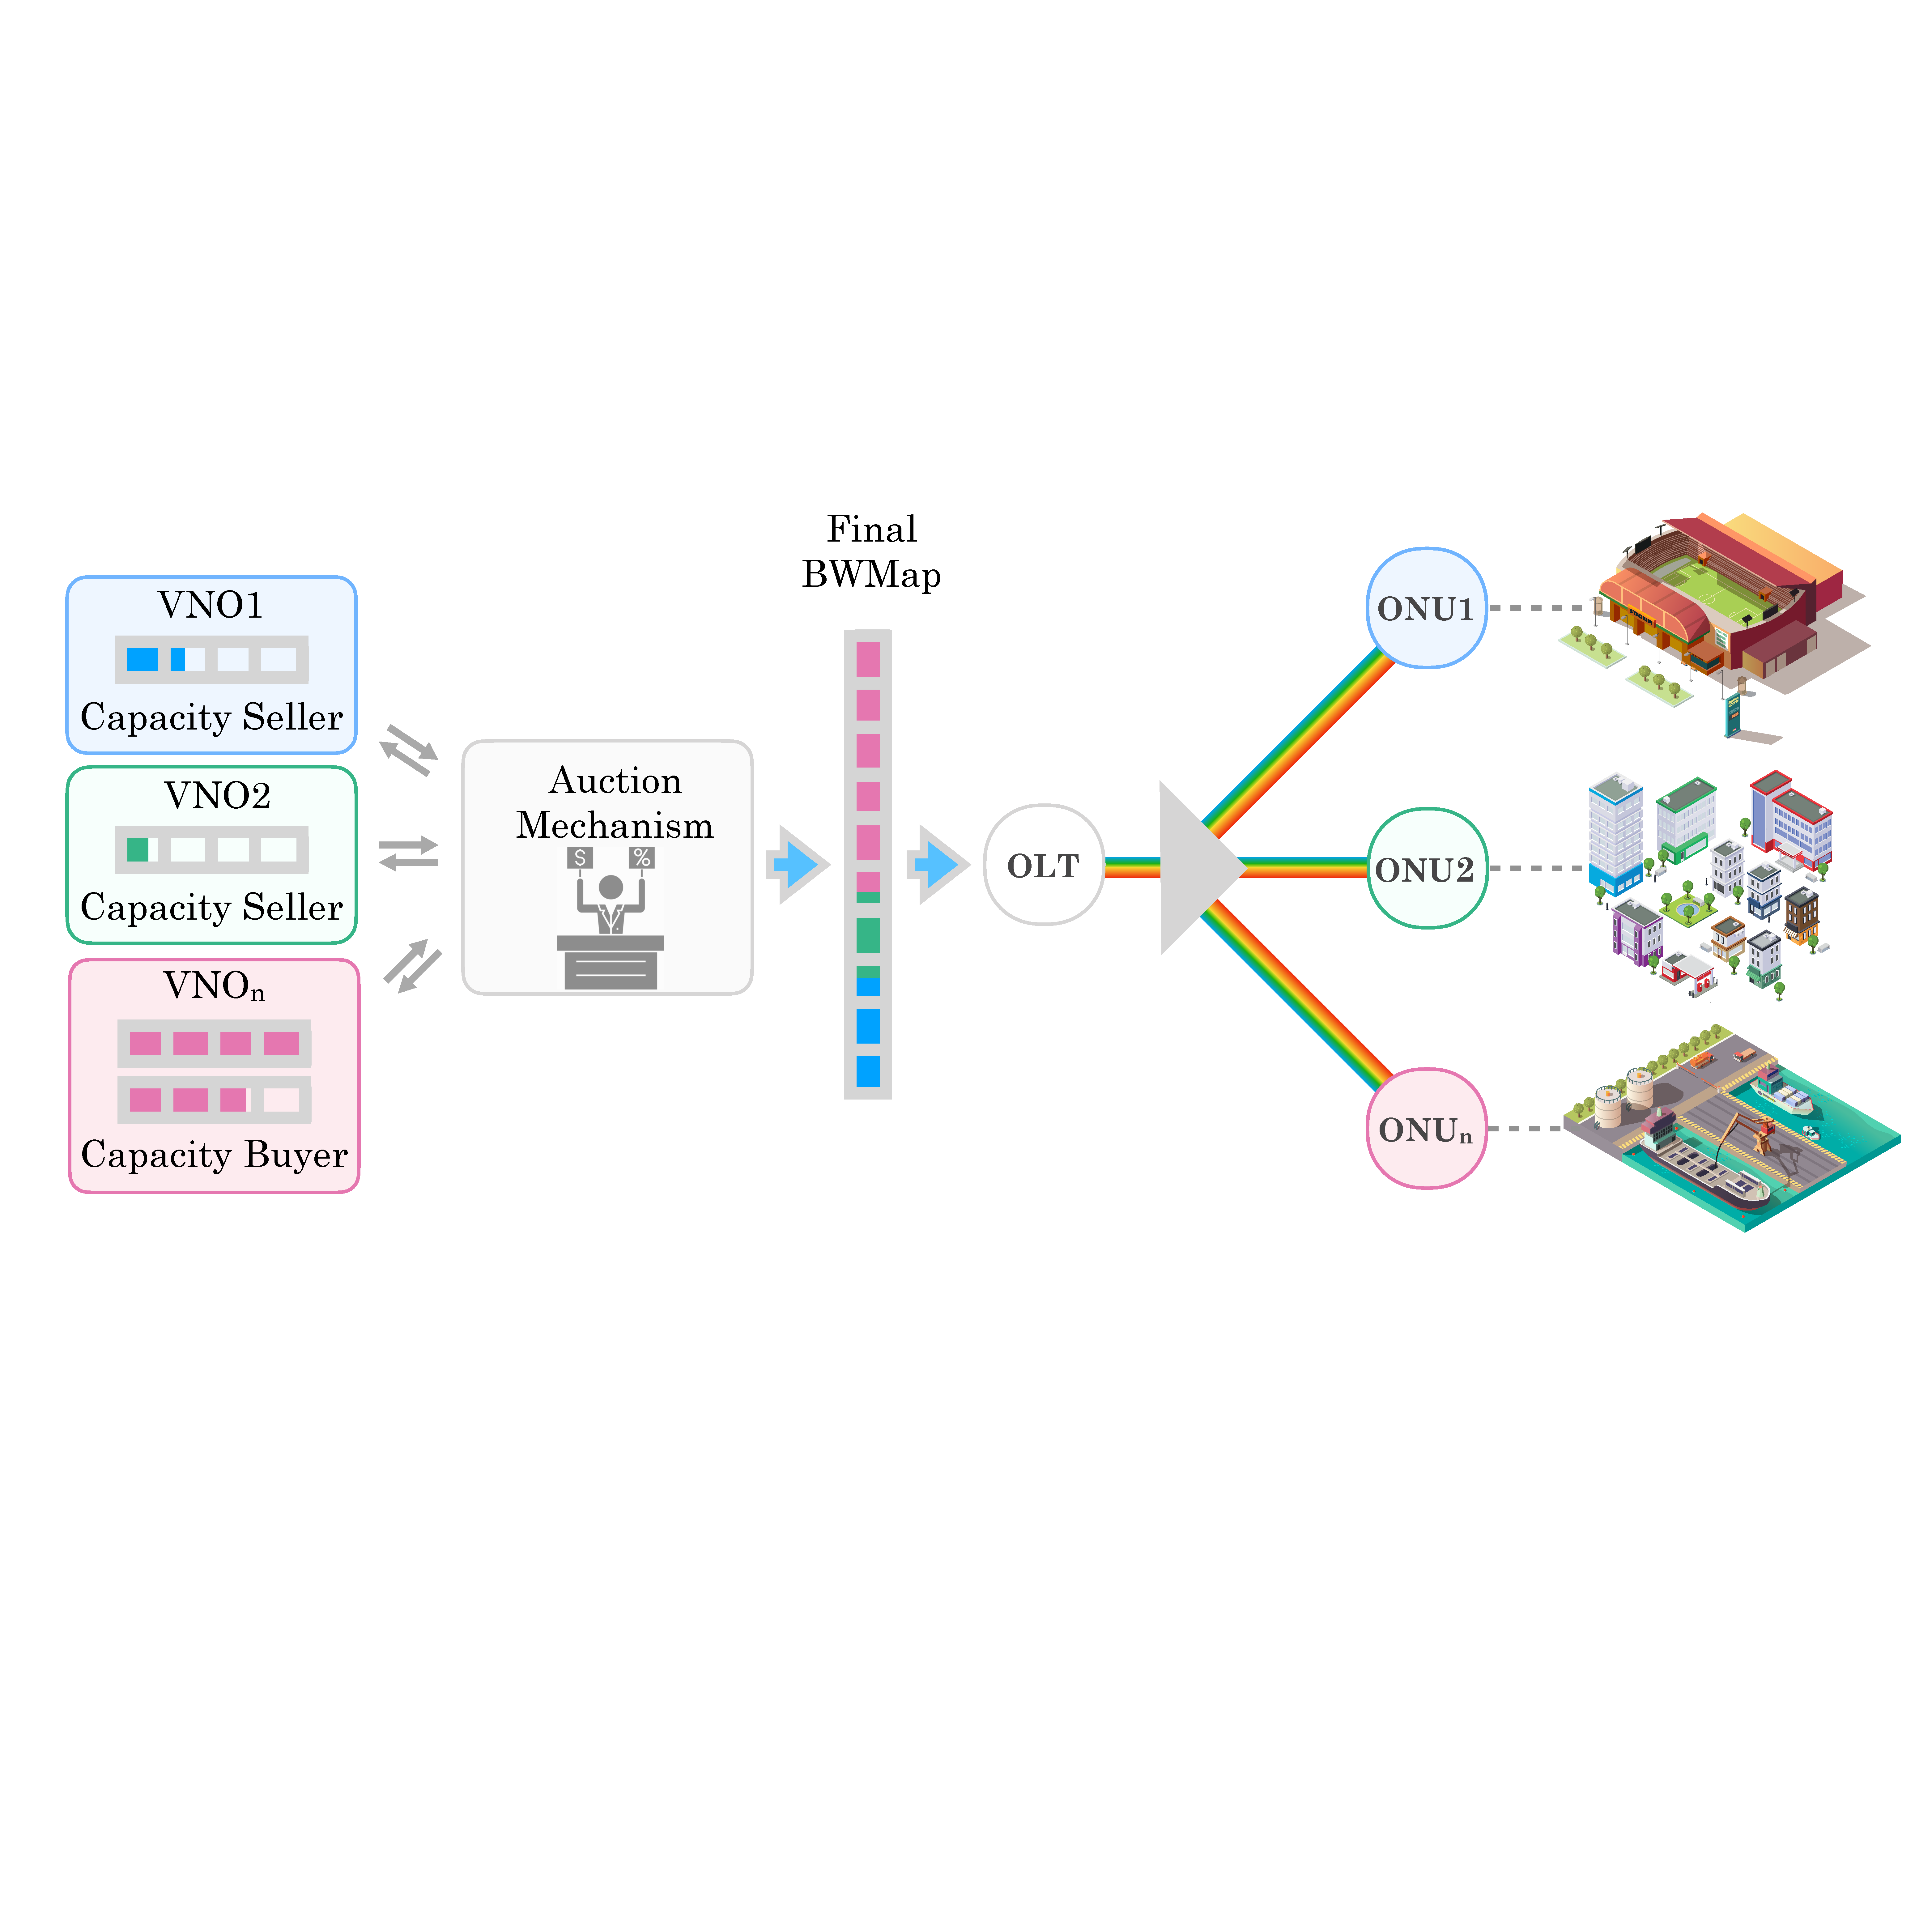
\includegraphics[width=\linewidth]{Figures/pon_new.pdf}
\caption{Multi-Tenant PON Sharing Market}
\label{market-fig}
\end{figure}
To address this obstacle, in \autoref{cpt:chapter_2} we introduce a marketplace (depicted in \figureautorefname~\ref{market-fig}), where the operators can receive monetary compensation in return for sharing their excess resources (upstream PON transmission capacity). We make use of an auction mechanism to ensure sharing incentives and satisfaction of the typical economic market properties, including truthfulness.
\toimprove{maybe more on blockchain}
% One issue that arises once the scheduling is passed to VNOs is that without proper incentives, VNOs have little motivation in sharing any unused capacity with other VNOs, making the overall PON inefficient. Indeed, once VNOs can fully control their slice scheduling their best strategy is to always pretend they need all the contracted capacity, which might otherwise be re-directed to a competing VNO.
% To address this challenge, we have proposed \cite{8386208} monetization of the excess PON slices where using an auction mechanism the VNOs can trade their excess capacity in return for monetary compensation (depicted in \figureautorefname~\ref{market-fig}). Through rigorous theoretical proofs and market simulations in \cite{Nima-JLT1} we validate that the proposed market will incentivize the VNOs to trade their excess resources in a setting where any attempt to manipulate the market will lead to worst or the same outcome.
% Nonetheless, the previous work assumes an open access architecture where a fully trusted central authority (Infrastructure Provider (InP)) is in charge of operating the market (bookkeeping, conducting the auction, settlements, etc.). This assumption may not be valid considering the new network ownership models. Hence, the natural progression of this work is to study distributed means of consensus (e.g., Blockchain-based Smart Contracts) which do not rely on a central entity. 
However, while the auction-based approach provides maintains high overall resource utilization, it does so under the assumption of an open-access architecture, where a fully trusted, independent central authority (e.g., the \ac{InP}) is in charge of operating the market (i.e., bookkeeping, conducting the auction, settlements, etc.). This assumption may not always be valid for today's network ownership models, where often the incumbent operator owning the physical infrastructure is also a competing \ac{VNO}.
We have thus tackled the more general problem of untrusted \ac{InP} through the use of distributed consensus mechanisms (e.g., Blockchain-based Smart Contracts), which do not rely on a central entity. %Our initial results \cite{Nima_globecom}, implemented over the Hyperledger Fabric \cite{Hyperledger}, showed that we could achieve more than 160 transactions (i.e., auction rounds) per second on a system with 8 virtual CPUs. This result already enables to carry out a capacity auction every 6 ms, i.e., averaged over about 50 frames. It is expected that transaction speed will further increase in the near future, as the Hyperledger Fabric community has recently set up a dedicated working group to address performance scalability \cite{pswg}. In addition, latest experiments \cite{fastfabric} have shown that performances of the order of 20,000 transactions per second are already possible for some types of applications in Hyperledger Fabric.

% In \cite{7936877} we studied two cases of capacity sharing from a technical perspective, to confirm its feasibility. However, in this work, no incentives for \acp{VNO} were considered for sharing their excess capacity.\\
% In \cite{1677253} the authors have proposed a dual service-level agreement to meet the fairness requirements for open access in a multi-tenant PON, mainly focusing on the fair allocation of the resources and neglecting the sharing incentives of the players. 
% In this paper, we will focus on the incentives of the market players while proposing an auction mechanism to choose the efficient trades and determine the pricing. To the best of the authors' knowledge, this paper is the first to study the sharing incentives in a multi-tenant \ac{PON} network.



% On the other hand in in a shared \ac{PON}  As an example, fiber infrastructure is inevitably the only long-term solution for mobile back/fronthaul \cite{6461186}. However 







% \towrite{Say we will waste BW if we use non-sharing}

% Considering the above argument, in a multi-tenant \ac{PON} scenario, a network operator may have a natural incentive to share the infrastructure with other operators in return for lower CAPEX and OPEX. Nevertheless, it should be taken into account that these network operators possibly are competing to gain more market share by increasing their customer base. Hence, without any incentives, \acp{VNO} will have no interest in re-distributing their unused capacity to other \acp{VNO} unless a business case guarantees a return on their "generosity". 
% \towrite{Say how we use monetization of resources to incentivize sharing}
% Thanks to the advances in optical networks technologies, the standardization bodies are moving toward higher rates for passive optical networks (PON). The IEEE 100G-EPON Task Force \cite{100g-epon} is aiming at 100 Gbit/s of capacity for its next-generation of \ac{PON} and the International Telecommunication Union's (ITU) NG-PON2 \cite{g.989.2} is already offering 80 Gbit/s capacity using Time and Wavelength Division Multiplexing (TWDM). \textcolor{blue}{However, the adoption of these technologies will greatly depend on the cost-reductive advances concerning the production of user-end equipment.}


% Currently, PONs are mainly dedicated to fiber to the home (FTTH) systems, e.g., for providing residential broadband. However, PONs have attracted interest from a diverse range of service providers (e.g., entities offering fifth generation (5G) mobile communications serivces, and Virtual Reality (VR) services \cite{8289443}) as they are interested in using the \ac{PON} as their access platform. The advantages that \ac{PON} offers compared to the other access solutions include high-capacity transmitting, lower CAPEX and OPEX costs compared to other alternatives such as point-to-point fiber as \ac{PON} enables multiplexing gains from sharing the fiber capacity between the optical network units (ONUs).


% In the context of optical access networks, such cost reduction can be achieved by increasing infrastructure utilization. One approach to sharing the infrastructure is the passive approach in which the operators share the site and the passive equipment. The second approach, which will be our primary focus in this research, is active infrastructure sharing, which enables improvements in network utilization by more fine-grained sharing models. For instance, sharing a \ac{PON} by dedicating a full wavelength channel to each different virtual network operator is possible using the currently available technologies. However, such coarse-grained sharing models impose boundaries on the extent of sharing, as it does not allow to utilize any unused capacity within each wavelength channel. Sharing the network at the sub-wavelength scale is thus important to fully exploit the advantages of multi-tenancy. 

% Traditional sharing models include sharing of capacity at higher layers, where for instance, a \ac{VNO} can collect traffic from its customers at a metro or regional aggregation point. This is the type of multi-tenancy service offered for example through bitstream. The main issue is its lack in flexibility as the \ac{VNO} can only offer very simple type of services to its customers, with little ability to differentiate its offer from its competitors, e.g., in terms of capacity, latency or quality of service. In short, current sharing models fail to provide the operators sufficient control over the shared infrastructure.




% The purpose of this document, therefore, is to explore the technical aspects associated with the application of virtualization and other suitable technologies to enhance access network sharing, in both brown-field and green-field situations, as network virtualization enables:
% • faster time to market and roll-out of new services
% • multi instance virtualization of access networks.
% It will identify the options available and provide a balance view on the pros and cons.

% FTTx represents today a future proof technology to enhance data rates to end customers. However, the deployment of FTTx may have a long RoI (Return on Investments) even for high take up rates. FTTx may require a major investment in \ac{CapEx} and \ac{\ac{OpEx}} for access network deployment.
% Some operators have recognized the need to partner to improve RoI of FTTx deployment. Partnerships and joint ventures are being formed between operators specifically for FTTx deployment. Sharing the network infrastructures (in particular the access network) is a viable way to expand the network and achieve an effective roll-out of new technologies.
% The main drawback with “bitstream” approach is that the architecture and all service designs have to be agreed in advance between the infrastructure provider and all involved operators. This is typically a long process that impacts the time to market for new services and features and therefore limits new service creation and evolution of the network. So in practice, only basic service offerings with minimal scope for differentiation can be delivered by hosted operators in a timely manner. A new collaboration model would allow hosted operators to have better control of resources rented from the operator owning the infrastructure and a higher degree of flexibility in service models.
% This study document provides a list of use cases with related high-level requirements that provides a framework defining an access network that can be shared among partner operators beyond traditional “bitstream” approach. It also proposes some sharing techniques that support all or part of use cases proposed.
% Finally the study document analyzes existing gaps in current and ongoing standards and includes recommendations for future work.



% \section{Research Gaps}
% \begin{itemize}
% \item The current sharing happens in higher network layers; therefore it is very coarse-grained (Packet-level). By moving the sharing closer to the physical layer, we can achieve more fine-grained sharing as there is more access to the network functions, e.g. frame-level scheduling.
% \item Lack of flexibility in the network functions which becomes essential as service diversity emerges.
% \item Lack of sharing incentives when the \acp{VNO} have to share their excess bandwidth with others.
% \end{itemize}

% \begin{enumerate}
% \item \ac{PON} is a good access solution i.e high capacity
% \item Thus can host more than one operator sharing
% \item Why is it important to share the PON?
%
%
% Infrastructure is cheaper so higher geographical coverage rural areas remote areas.
% %This can even become a racial issue as some remote suburban areas might be populated with people with a special ethnic background etc.
% Disadvantaged neighborhood, Developing countries can cause socio-economical problems.  Article 19 of the Universal Declaration of Human Rights communication basic-fundamental human right.
%
% \item new small operators market more competitive (new network ownership/operation models)
%
% \item Service providers are already becoming (virtual) network operators. Examples:
% \item Google Fiber
% \item Facebook Africa cable https://goo.gl/sRXQnD
% \item \textbf{Obstacles:}
% \item so we have to make the \ac{PON} DBA flexible so it can support new emerging services it flexible
% \item Can we design a mechanism which is economic-robust without loosing too much efficiency?
% \item It can host multiple traditional broadband operators alright.
% \item However new emerging services have more strict requirements
% \item such as latency in C-RAN and VR and some that we have not seen yet
% \item BUT current \ac{PON} can't support the requirements of the new emerging services.
% \item Why?
% \item Because DBA is slow and it's hard-coded and not flexible
%
% \end{enumerate}


\section{Key Contributions}
In the study of the technological and economic enablers of optical network sharing the following primary contributions are made:

\subsection{True \ac{PON} Multi-Tenancy Enabled by \ac{DBA} Virtualization}
\begin{itemize}

\item Enabling true and flexible multi-tenant \ac{PON} architecture by providing the operators with more control over their share of the resources. This is achieved by providing a virtual hence customizable instance of the \ac{DBA} as opposed to the hard-coded \acp{DBA} in conventional \ac{PON} architecture.


\end{itemize}
\subsection{Designing a Market Model for Multi-Tenant \ac{PON}s}
\begin{itemize}

\item This is to design a market model for the multi-tenant \ac{PON} market that incentivizes the tenants to willingly participate in resource sharing to achieve a common objective, which is reducing the infrastructure costs and facilitate the widespread network coverage.

\item In the proposed market model, the network tenants are compensated monetarily in return for sharing their idle share of the network with others. The model depends on a central trusted entity that is responsible for book-keeping and processing the market.


\end{itemize}
\subsection{Developing an Efficient and Economic-Robust Auction Mechanism for \ac{PON} Sharing Market}
\begin{itemize}


\item We proposed a new sealed-bid, multi-item, \textit{double auction} mechanism to efficiently allocate the resources while maximizing the social welfare of the market. We have proven that our proposed algorithm is compatible with the VNOs' incentives and guarantees positive a budget for the InP.


\item We proposed a trade reduction mechanism that scarifies fewer trades to achieve the crucial economic properties. These achievements are reached while the mechanism adds no additional communication overhead to the system due to its single rounded nature.


\end{itemize}

\subsection{Distributed Network Sharing Market Ecosystem}
\begin{itemize}


\item We challenge the assumption of the centrally trusted market holder, where we discussed how this could be unrealistic. We further provided an initial review of the potential solutions to this problem for future work.


\end{itemize}


%%%%%%%%%%%%%%%%%%%%%%%%%%%%%%%%%%%%%%%%%%%%%%%%%%%%
%%%%%%%%%%%%%%%%%%%%%%%%%%%%%%%%%%%%%%%%%%%%%%%%%%%%
%%%%%%%%%%%%%%%%%%%%Dissemination%%%%%%%%%%%%%%%%%%%
%%%%%%%%%%%%%%%%%%%%%%%%%%%%%%%%%%%%%%%%%%%%%%%%%%%%
%%%%%%%%%%%%%%%%%%%%%%%%%%%%%%%%%%%%%%%%%%%%%%%%%%%%

\section{Structure}

\tochange{Update the structure at the end}
The Structure of this thesis is as follows:
    \begin{itemize}
    %   \item In Chapter \ref{Chap:PON}, we give a brief overview of the \ac{PON} and the Dynamic Bandwidth Allocation (DBA) in section.
    \item \autoref{cpt:background} provides an introduction along with a state-of-the-art review of the underlying concepts addressed in this thesis. It begins with an introduction to \acp{PON} (\autoref{Back:Sec:PON}) as the main access network solution under the study in this thesis and its crucial \ac{DBA} function (\autoref{Back:Sec:PON:sub:DBA}). In \autoref{Back:Sec:sharing} we introduce network sharing as the main scope of this thesis while elaborating on market players aggressive competition policies and the emerging network ownership models (\autoref{Back:Sec:sharing:sub:competition}) that are born out of such market dynamics. 
    In \autoref{Back:Sec:Virtualazation}, we provide some background for network virtualization and related technologies while showing how they can facilitate network sharing. A brief literature review on the auction theory and in particular double auctions is provided in \autoref{Back:Sec:auction}. Finally, in \autoref{Back:Sec:blockchain}, we provide the necessary background for blockchain and smart contract technology with a focus on their application in communications and distributed market mechanisms. 
    
    \item In \autoref{cpt:methodology} we outline the research questions addressed in this thesis and discuss the methods used to design experiments and evaluate the solutions proposed by the contributions of this thesis. 
    % We will then describe the desirable economic properties of the market and their relationship with the utility functions of the agents.
    
    \item In \autoref{cpt:chapter_1} addresses the technological barrier of multi-service optical access sharing by introducing a new architecture for multi-tenant \acp{PON}, which enables customized resource allocation for the tenant operators.
    
    
    \item In \autoref{cpt:chapter_2} we model the multi-tenant \ac{PON} network as a market (\autoref{sec:market-model}) while introducing the roles of the agents involved in the market. We further propose an auction mechanism (\autoref{sec:auction_mechanism}) to enable bilateral trade in the multi-tenant \ac{PON} market. Theoretical proofs for the satisfaction of the economic properties and the analysis of the allocative efficiency of the proposed mechanisms are also provided in this chapter.
    \item In \autoref{cpt:chapter_3}, a distributed market mechanism based on permissioned blockchain technology, is introduced. The proposed distributed mechanism implemented using the smart contract technology is then applied to two different scenarios, including the multi-tenant \ac{PON} and \ac{5G} slicing. The cloud-based implementation and deployment of the market are cover in this chapter. The blockchain-based solution is evaluated in terms of transaction throughput, latency, and required additional computational resources.
    
    
    % We use the Hyperledger Fabric blockchain framework to implement our solution, which has a considerably lower cost in terms of latency and computing compared to the traditional blockchain (e.g., Bitcoin). Our mechanism supports millisecond-level granularity capacity auctioning, enabling next-generation low-latency services to run in shared trust-less environments.
    
    \item Concluding remarks are given in \autoref{cpt:conclusion} along with a discussion of limitations and future work.
    
    
    % The main contributions of this paper are as follow:
    % \begin{enumerate}
    % \item We propose using auctions for resource allocation of multi-tenant optical networks. To the best of our knowledge, this is the first time that this approach is used. 
    % \item We propose a multi-item double auction mechanism that while maintaining the typical desired economic properties for a market place (details are provided in section \ref{Fig_model}), achieves a higher allocative efficiency when compared with state of the art mechanisms used in wireless spectrum sharing \cite{5462277}.
    % \end{enumerate}
    
    %   \item Concluding remarks are given in Chapter \ref{Chap:Conclusions} along with a discussion of limitations and future work.
    \end{itemize}



\section{Dissemination}
% \nobibliography{bib/thesis.bib}
% \bibliographystyle{IEEEtran}
% \bibliographystyleNew{IEEEtran}
% \nobibliography{bib/MyPub.bib}
% \nociteNew{Nima-globecom}
\nobibliography*
%%%%%%%%%%%%%%%%%%%%%%%%%%%%%%%%%%%%%%%%%%%%%%%%%%%%
% As an Alternative I can copy and paste from .bbl file.
%%%%%%%%%%%%%%%%%%%%%%%%%%%%%%%%%%%%%%%%%%%%%%%%%%%%

\subsection{Peer-Reviewed}

 \begin{enumerate}
    \item M. Ruffini, A. Ahmad, S. Zeb, \textbf{\underline{N. {Afraz}}}, and F. Slyne, “The Virtual DBA: Virtualizing Passive Optical Networks to Enable Multi-Service Operation in True Multi-Tenant Environments,” J. Opt. Commun. Netw., Jan. 2020.
    
    \item  \textbf{\underline{N. {Afraz}}} and M.~{Ruffini}, ``A Distributed Bilateral Resource Market Mechanism for Future Telecommunications Networks,'' in \emph{2019 IEEE Global Communications Conference (GLOBECOM)}, December 2019.

    \item \textbf{\underline{N. {Afraz}}}, F.~Slyne \emph{et~al.}, ``Evolution of Access Network Sharing and Its Role in 5G Networks,'' \emph{Applied Sciences}, vol.~9, no.~21, p. 4566, oct 2019.

    \item H.~Ahmadi, I.~Macaluso, M.~{Ruffini}, \textbf{\underline{N. {Afraz}}}, ``Blockchain Technology and Smart Contracts in 5G and Beyond Networks [Tutorial Talk],'' 2019, European Conferences on Networks and Communications (EUCNC).

    \item \textbf{\underline{N. {Afraz}}} and M.~{Ruffini}, ``A Sharing Platform for Multi-Tenant PONs,'' \emph{Journal of Lightwave Technology}, vol.~36, no.~23, pp. 5413--5423, Dec 2018.

    \item \textbf{\underline{N. {Afraz}}} and M.~{Ruffini}, ``A Marketplace for Real-Time Virtual PON Sharing,'' in \emph{2018 Asia Communications and Photonics Conference (ACP)}, Oct 2018, pp. 1--3.

    \item \textbf{\underline{N. {Afraz}}}, A.~{Elrasad}, M.~{Ruffini}, ``DBA Capacity Auctions to Enhance Resource Sharing Across Virtual Network Operators in Multi-Tenant PONs,'' in \emph{2018 Optical Fiber Communications Conference and Exposition (OFC)}, March 2018.
   
    \item \textbf{\underline{N. {Afraz}}}, A.~{Elrasad}, H.~Ahmadi,  M.~{Ruffini}, ``Inter-Operator Dynamic Capacity Sharing for Multi-Tenant Virtualized PON,'' in \emph{2017 IEEE 28th Annual International Symposium on Personal, Indoor, and Mobile Radio Communications (PIMRC)}, Oct 2017, pp. 1--6.

    \item A.~{Elrasad}, \textbf{\underline{N. {Afraz}}}, H.~Ahmadi , ``Virtual Dynamic Bandwidth Allocation Enabling True PON Multi-Tenancy,'' in \emph{2017 Optical Fiber Communications Conference and Exhibition (OFC)}, March 2017, pp. 1--3.


    % \item \bibentry{Nima-globecom}
    % \item \bibentry{Nima-5g-evol}
    % \item \bibentry{Nima-EUCNC-BC-Talk}
    % \item \bibentry{Nima-JLT1}
    % \item \bibentry{Nima-ACP}
    % \item \bibentry{Nima-OFC18}
    % \item \bibentry{Nima-PIMRC17}
    % \item \bibentry{Nima-OFC17}
 \end{enumerate}
 \subsection{Non Peer-Reviewed}
 \begin{enumerate}

    \item \textbf{\underline{N. {Afraz}}}, V.~Chaudhary \emph{et~al.}, ``Optimizing Wholesale Intercarrier Settlement with Hyperledger Fabric Blockchain,'' in \emph{Solution Brief}.\hskip 1em plus 0.5em minus 0.4em\relax Telecom Special Interest Group, 2019.

    \item \textbf{\underline{N. {Afraz}}}, F.~Slyne, M.~Ruffini, ``Full PON Virtulisation Supporting Multi-Tenancy Beyond 5G,'' in \emph{OSA Advanced Photonics Congress (AP) 2019 (IPR, Networks, NOMA, SPPCom, PVLED)}.\hskip 1em plus 0.5em minus 0.4em\relax Optical Society of America, 2019, p. NeT2D.2.


    % \item \bibentry{Nima-telecom-sig}
    % \item \bibentry{Nima-osa}
 \end{enumerate}
 \subsection{Patent}
    \begin{enumerate}
    \item M.~Ruffini, A.~Elrasad, \textbf{\underline{N. {Afraz}}}, ``System and {Method} for {Dynamic} {Bandwidth} {Assignment} (DBA) {Virtualization} in a {Multi}-{Tenant} {Passive} {Optical} {Network},'' Patent WO/2018/167\,318, Sep., 2018.
    %   \item \bibentry{Nima-vDBA-patent}
    \end{enumerate}


% \nocite{*}
% \bibliographystyle{IEEEtran}
% \renewcommand\bibname{}
% \bibliography{bib/MyPublications}

% \printbibliography[title={Reference}]

%-------------- BIBLIOGRAPHY -----------------------
% hack pagestyle
% \fancypagestyle{empty}{\pagestyle{bibmine}}

% \begin{singlespacing}
%     \cleardoublepage\pagestyle{bibmine}%
%     \phantomsection%
%     \addcontentsline{toc}{chapter}{Bibliography}%
%     %\bibliographystyle{IEEEtranmineS} %abbrvnat}%siam, ifac  %acm, ieeetr, phjcp
%     \bibliographystyle{IEEEtran}
%     \bibliography{bib/MyPublications}
% \end{singlespacing}